% (c) Egor Osipov

\documentclass[a4paper,12pt]{article} % тип документа (report, book)
\usepackage[left=2cm,right=2cm, top=2cm,bottom=2cm,bindingoffset=0cm]{geometry} % Настройки документа


%  Русский язык
\usepackage[T2A]{fontenc}			% кодировка
\usepackage[utf8]{inputenc}			% кодировка исходного текста
\usepackage[english,russian]{babel}	% локализация и переносы


% Математика
\usepackage{amsmath,amsfonts,amssymb,amsthm,mathtools} 

% Просто смайлики
\usepackage{wasysym}

%Вставка картинок
\usepackage{graphicx}
\graphicspath{./}
\DeclareGraphicsExtensions{.pdf,.png,.jpg}
\usepackage{float}

% Настройка абзацев
\usepackage{indentfirst}
%\setlength{\parindent}{5ex}
%\setlength{\parskip}{1em}

\begin{document} % начало документа

%Заговолок
\begin{titlepage}
\begin{center}
	\large{Московский физико-технический институт}\\
	\vspace{100px}
	\LARGE{Лабораторная работа № 3.2.4}\\
	\LARGE{Свободные колебания в электрическом контуре.}\\
	\vspace{30px}
	
\includegraphics[scale = 0.3]{fakt_logo.png}\\
\end{center}

\vfill
\begin{flushright}
	\text{Осипов Егор. Б03-005}\\
	\text{07.09.2021}\\
	\text{г. Долгопрудный}
\end{flushright}
\end{titlepage}

\newpage

\tableofcontents

\newpage

\textbf{Цель работы:} исследование свободных колебаний в колебательном контуре.

\textbf{В работе используется:} Генератор импульсов, электрическое реле, магазин сопротивлений, магазин емкостей, индуктивность, электронный осциллограф, универсальный мост.

\begin{center}
\section{Экспериментальная установка}
\end{center}

\begin{figure}[h]\label{ustanovka}
	\center{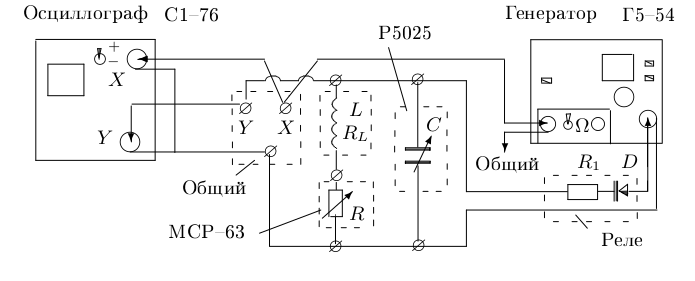
\includegraphics[scale=0.7]{ustanovka}}
	\caption{Схема установки для исследования свободных колебаний}
\label{fig:image}
\end{figure}

\begin{center}
\section{Ход работы}
\end{center}


\subsection{Подготовим установку к работе.}

Для этого у нас уже собрана схема, изображенная на рисунке (1).\\
Ручкой АМПЛ генератора импульсов установим напряжение на вольтметре чуть больше 30 В. Установим длительность импульсов $\sim 5$мкс.Частоту повторения -- $\nu_0 = 100$Гц.

\subsection{Измерение периодов}

1. Установим на магазине сопротивлений сопротивление R = 0; на магазине емкостей величину C = 0.02мкФ\\

2. Прокалибруем горизонтальную ось осциллографа по известному периоду импульсов:

a) подберем частоту осциллографа при которой расстояние $x_0$ между импульсами, поступающими с генератора ($T_0 = 0.01$с), занимает почти весь экран.

б) измерив на экране расстояние $x$, которые занимают несколько полных периодов \textit{n}, рассчитаем период колебаний контура: $T = T_0x/(nx_0)$. Малые расстояния будем увеличивать.

Результаты занесем в таблицу \eqref{table1:ref}.

\begin{table}[H]
\caption{\label{tab:canonsummary} Измерение периода.}
\begin{center}
\begin{tabular}{|c|c|c|c|c|c|}
\hline
n & $x_0$ ($*10^{-3}$сек) & $x$ ($*10^{-3}$сек) & $T_\text{теор}$ ($* 10^{-2}$сек) & С ($*10^{-6}$Ф)&$T_\text{эксп}$ ($* 10^{-2}$сек)\\
\hline
5 & 10 & 1.74 & 0.35 &0.02 & 0.40\\
\hline
3 & 9.8 & 2.5 & 0.85 &0.12 & 0.97\\
\hline
4 & 9.8 & 4.5 & 1.1 &0.22 & 1.32\\
\hline
3 & 9.8 & 4.1 & 1.4 &0.32 & 1.59\\
\hline
3 & 9.8 & 4.65 & 1.58 &0.42 & 1.82\\
\hline
2 & 9.8 & 3.45 & 1.76 &0.52 & 2.03\\
\hline
4 & 9.8 & 7.5 & 1.91 &0.62 & 2.21\\
\hline
3 & 9.8 & 6 & 2.04 &0.72 & 2.38\\
\hline
3 & 9.8 & 6.6 & 2.24 &0.82 & 2.54\\
\hline
3 & 9.8 & 6.8 & 2.31 &0.9 & 2.66\\
\hline
3 & 9.8 & 6.7 & 2.27 &0.86 & 2.60\\
\hline
\end{tabular}
\end{center}
\label{table1:ref}
\end{table}

\subsection{Критическое сопротивление и декремент затухания}

1. Приняв L=200мГн, рассчитайте емкость C, при которой собственная частота колебаний контура $\nu_0 = 1/(2\pi\sqrt{LC})$ совставляет 5кГц. После для выбранных значений L и C рассчитаем критическое сопротивление контура $R_{crit}$ по формуле \eqref{2.20}.

\begin{equation}\label{2.20}
R_{crit} = 2\sqrt{\frac{L}{C}}
\end{equation}

2. Далее найдем экспериментально значение $R_{ex}$. Для этого будем изменять значение сопротивления от 0 до $R_{crit}$

3. Установим сопротивление $R \simeq 0.1R_{exp}$. Получим на экране картину затухающих колебаний. Для расчета \textbf{логарифмического декремента затухания} по формуле \eqref{2.30} измерим амплитуды, разделенные целым числом периодов. Измерения повторим 5-6 раз.

\begin{equation}\label{2.30}
\Theta = \frac{1}{n}\ln \frac{U_k}{U_{k+1}}
\end{equation}

%\subsection{Колебания на фазовой плоскости.}
%
%1. Поставим рычаг переключения разверстки осциллографа в положение <<X>>.\\
%При значении $C = 5 \cdot 10^{-9}$Ф пронаблюдаем за изменением спирали при увеличении сопротивления от $0.1 \cdot R_{crit}$ до $0.3 \cdot R_{crit}$.\\
%Для измерения $\Theta$ измерим радиусы витков спирали при нескольких значениях сопротивления.\\
%
%2. Измерим индуктиность \textit{L} и омическое сопротивление катушки $R_L$ с помощью моста переменного тока.

\begin{center}
\section{Обработка результатов}
\end{center}

1. Рассчитаем экспериментальные значения периодов по результатам измерений  2.2.2 и теоритические по формуле \eqref{2.21}. Построим график $T_{exp} = f(T_{teor})$.

\begin{equation}\label{2.21}
T = \frac{2\pi}{\omega_0} = 2\pi \sqrt{LC}
\end{equation}

\begin{figure}[H]\label{periods}
	\center{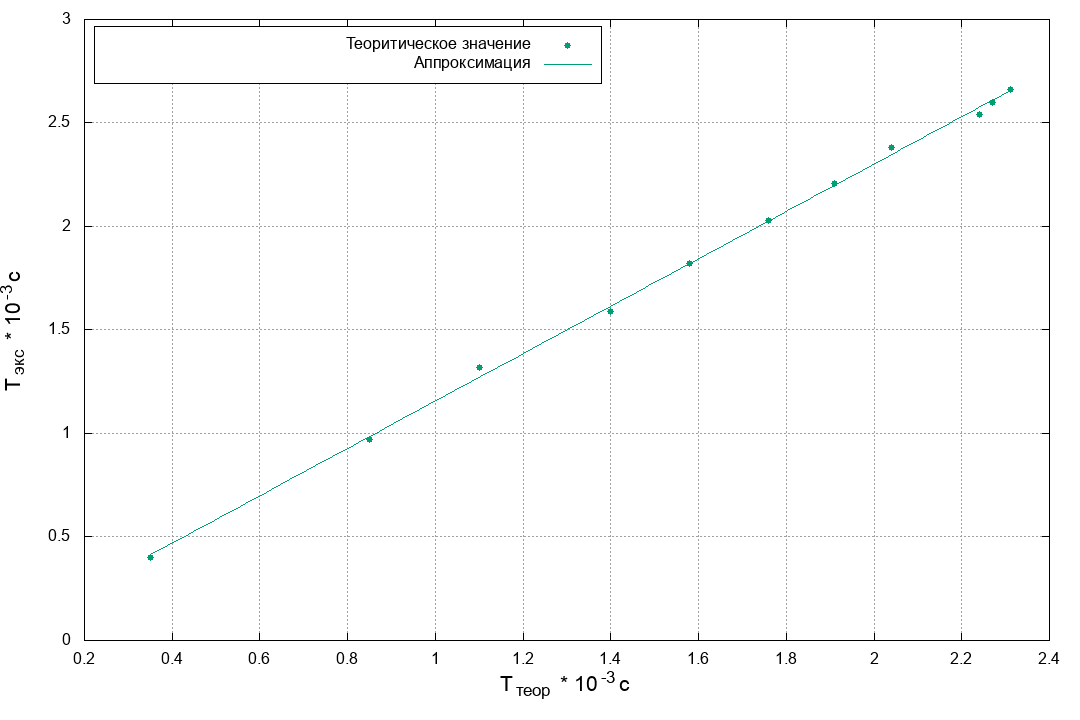
\includegraphics[scale=0.6]{./data/translated/periods}}
	\caption{График зависимости экспериментального значения периода от теоритического.}
\label{fig:image}
\end{figure}

Наклон графика получился $k = 0.87 \pm 0.01$, что означется, что брать $L = 200$мГн слишком оптимистично. Из уравнения \eqref{2.21} можно найти удовлетворяющую нас величину: $L = 150.7 \pm 0.5 \text{мГн}.$

Емкость, при которой собственная частота колебаний составляет 5кГц:

\begin{equation}
    C = \frac{1}{4\pi^2{\nu_0}^2L} = 5*10^{-9} \text{Ф}
    \label{eq2:ref}
\end{equation}

$R_\text{crit}^\text{exp} = 8.6 \text{кОм}$

$R_{\text{кат}} = 10.7 \text{Ом}$ при частоте колебаний в 5 кГц. 

\begin{equation}
    \Theta = \frac{1}{n}ln\left(\frac{U_k}{U_{k+n}}\right)
    \label{eq4:ref}
\end{equation}

2. Рассчитаем значения $\Theta$ и $R_{cont}$ (сопротивление контура, которое состоит из сопротивления магазина и сопротивления катушки). Значения занесем в таблицу \eqref{tab:canonsummary}

\begin{table}[H]
\caption{\label{tab:canonsummary} Измерение логарифмического декремента затухания.}
\begin{center}
\begin{tabular}{|c|c|c|c|c|}
\hline
$R_\text{конт} \text{(кОм)}$ & $U_1$ (дел) & $U_2$ (дел) & n & $\Theta$\\
\hline
0.87 & 3 & 0.2 & 5 & 0.54\\
\hline
1.01 & 2.9 & 0.2 & 4 & 0.67\\
\hline
1.31 & 2.6 & 0.2 & 3 & 0.85\\
\hline
1.71 & 3.2 & 0.4 & 2 & 1.04\\
\hline
2.01 & 2 & 0.2 & 2 & 1.15\\
\hline
2.31 & 4.2 & 0.2 & 2 & 1.52\\
\hline
\end{tabular}
\end{center}
\label{table2:ref}
\end{table}

3. Построим график в координатах $1 / \Theta^2 = f(1 / R^2_{cont})$ (Рисунок (3)). Определим критическое сопротивление $R_{crit}$ по наклону прямой, приняв обозначения $1/\Theta^2 = Y$, $1 / R^2_{cont} = X$, можно показать, что:

\begin{figure}[h]\label{theta_graph}
	\caption{График зависимости обратной величины квадрата логарифмического декремента затухания от обратной величины квадрата сопротивления контура.}
	\center{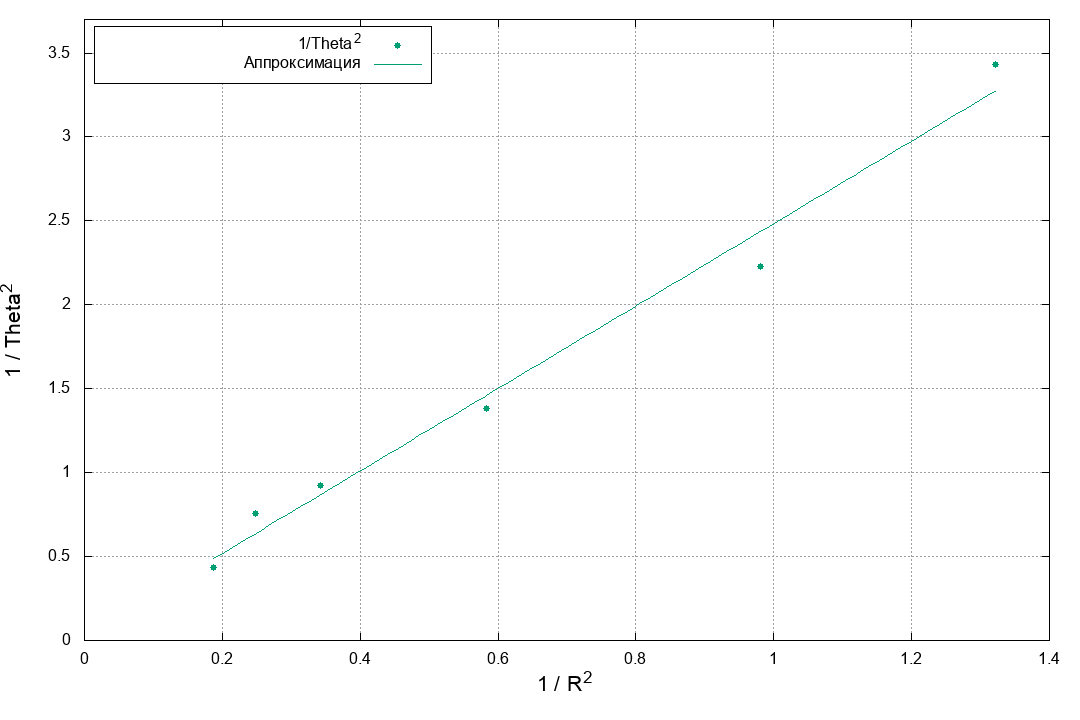
\includegraphics[scale=0.6]{./data/translated/theta}}
\label{fig:image}
\end{figure}

\begin{equation}\label{2.100}
R_{crit} = 2\pi \sqrt{\frac{\bigtriangleup Y}{\bigtriangleup X}}
\end{equation}

Из графика получаем $\frac{\Delta Y}{\Delta X} = 2.45$. $ R_\text{crit} = 2\pi\sqrt{\frac{\Delta Y}{\Delta X}} = 9.83 \pm 0.12 \text{кОм} $

4. Рассчитаем $R_{crit}$ по формуле \eqref{2.20} и сравним результаты: теоритический, графический и экспериментальный и сведем все в таблицу \eqref{tab:compilation}.

\begin{equation}
    R_\text{crit} = 2\sqrt{\frac{L}{C}} = 10.98 \text{кОм}
    \label{eq5:ref}
\end{equation}

\begin{table}[H]
\caption{\label{tab:compilation} Сравнение разных методов измерения критического сопротивления.}
\begin{center}
\begin{tabular}{|c|c|}
\hline
& $R_\text{крит}$ кОм\\
\hline
Теоритический & 10.98\\
\hline
Графический & 9.83 $\pm$ 0.12 \\
\hline
Экспериментальный & 8.6\\
\hline
\end{tabular}
\end{center}
\label{table3:ref}
\end{table}

5. Рассчитаем добротность контура для максимального и минимального значений $\Theta$, используя равенства \eqref{2.30} и \eqref{2.31} и сравним с расчетом \textit{Q} через параметры R, C, L по формуле \eqref{2.28}. Сведем все в таблицу \eqref{tab:canonsummary}.

\begin{equation}\label{2.28}
Q = \frac{1}{R} \sqrt{\frac{L}{C}}
\end{equation}

\begin{equation}\label{2.31}
Q = \frac{\pi}{\gamma T} = \frac{\pi}{\Theta}
\end{equation}

\begin{table}[H]
\caption{\label{tab:canonsummary} Измерение добротности.}
\begin{center}
\begin{tabular}{|c|c|c|c|c|c|c|}
\hline
$\Theta$ & $Q_\text{экс}$ & R (кОм) & L (мГн) & C (пФ) & $Q_\text{теор}$ & $\Delta$ Q\\
\hline
0.54 & 5.82 & 0.86 & 150.7 & 5 & 6.38 & 8.77\%\\
\hline
1.52 & 2.07 & 2.3 & 150.7 & 5 & 2.39 & 13.3\%\\
\hline
\end{tabular}
\end{center}
\label{table4:ref}
\end{table}

6. В таблицу \eqref{tab:theta_circus} сведем зависимость омического сопротивления от частоты.

\begin{table}[H]
\caption{\label{tab:theta_circus} Зависимость омического сопротивления от частоты.}
\begin{center}
\begin{tabular}{|c|c|c|c|}
\hline
& 50 Гц & 1 кГц & 5 кГц\\
\hline
$R_{cat}$ (Ом) & 10.4 & 11.2 & 10.7\\
\hline
L (мГн) & 145 & 141.35 & 141\\
\hline
\end{tabular}
\end{center}
\label{table5:ref}
\end{table}

\begin{center}
	\section{Вывод.}
\end{center}

В процессе работы были исследованы свободные колебания в электрическом контуре. Были найдены добротность колебаний и логарифмический декремент затухания $\Theta$.
\end{document} % конец документа